\chapter{Introduction}
	\label{chap:intro}
	
\section{Adversarial attacks}
    \label{sec:introduction}

Over the past 10 years, deep neural network models have advanced tremendously, with numerous novel architectures being proposed \cite{alexnet, densenet, googlenet}. They have been used for tasks such as object recognition, image segmentation, automatic language translation, and safety and security-critical tasks, such as face recognition \cite{face_recognition}, self-driving cars \cite{self_driving_cars} and malware detection \cite{malware_detection}. 

However, neural networks are vulnerable to a variety of attacks which enable malicious agents to manipulate their outputs \cite{deep_leakage, trojan_attacks, poisoning_attacks, szegedy2014intriguing}, including adversarial attacks. First discovered in 2014 by Szegedy \textit{et al.} \cite{szegedy2014intriguing}, they involve crafting special perturbations that are added to the original input to make the victim model output a wrong label. Moreover, these perturbations are often imperceptible to humans \cite{szegedy2014intriguing}, and can specific wrong outputs which are very different to the correct output.

Since then, research has proven that attacks in the physical world \cite{evtimov_road_signs} and in cyberspace \cite{papernot_cyberspace_attack} are possible. For example, Eykholt \textit{et al.} \cite{evtimov_road_signs} successfully performed an adversarial attack that fooled a road sign recognition model in real life. Athalye \textit{et al.} \cite{athalye} created physical 3D objects that consistently fool image recognition NNs, regardless of the camera angle. This was in contrast to traditional attacks that create 2D adversarial images, as those are much less effective when printed and physically held in front of a camera \cite{lu_physical_experiments}. Consequently, the existence of adversarial examples undermines the applicability of neural networks, especially in domains where safety is critical.

One disadvantage of the physical world attack created by Athalye \textit{et al.} is that it is a \textbf{white-box} attack, it requires access to the targeted model. Another line of research looked at \textbf{black-box} attacks, which do not have this requirement \cite{akhtar} and are thus more practical for the attackers. However, the black-box attacks in the literature only create 2D adversarial examples in the lab setting and are much less effective in a physical scenario.

An adversarial attack that is both black-box and applicable to the physical domain would be especially practical for attackers, and thus dangerous. Therefore, my project will try to combine the framework used in Athalye \textit{et al.} \cite{athalye} and the generative model presented in \cite{zheng_black_box_GAN} to create a black-box adversarial attack which produces 3D rendered objects that can consistently fool object classifier neural networks. The project is exploratory in nature and seeks to investigate if such an attack is possible. The findings, such as fooling rates against various victim models, may be useful for further understanding the nature of adversarial attacks and for creating better defence methods.

\section{Motivation}
    \label{sec:motivation}
	
Adversarial attacks are often highly effective at fooling a victim model \cite{akhtar, silva_survey, dong2020benchmarking, robustart, fgsm}. One dangerous example was demonstrated in Hendrik Metzen \textit{et al.} \cite{Metzen_2017_ICCV}, where the authors performed adversarial attacks on a neural network used for image segmentation for use in a self-driving car. They managed to make the victim model not perceive pedestrians, as 84.5\% of pedestrian pixels were misclassified. If an attacker were to implement it in real life, the self-driving car could have run over pedestrians, as it would not see them, as you can see in figure \ref{fig:adversarial_segmentation}. However, the attacks in \cite{Metzen_2017_ICCV} were only done in a lab setting and not a physical setting.

\begin{figure}[ht]
    \centering
    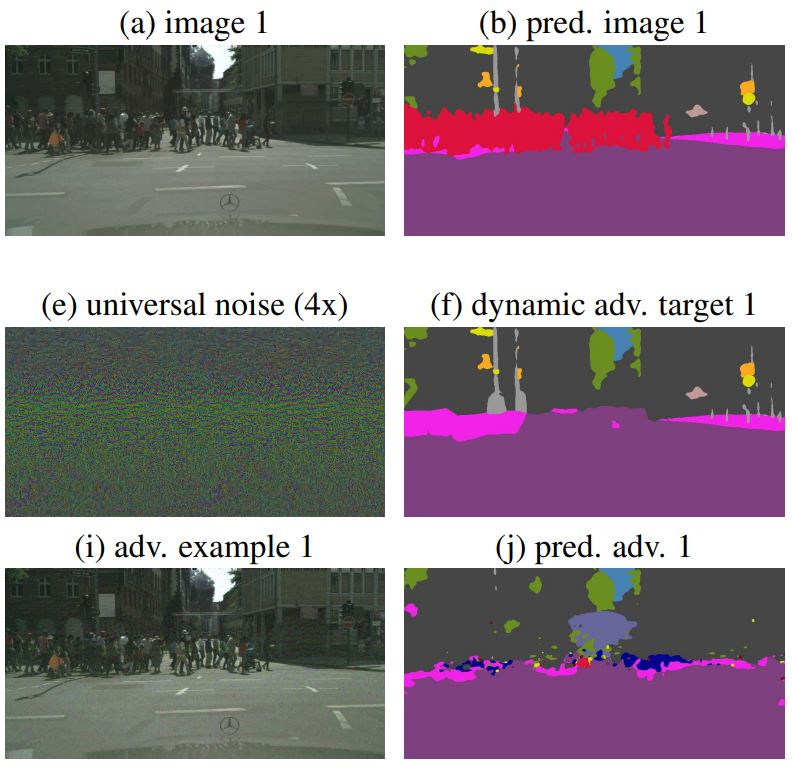
\includegraphics[width=0.8\textwidth]{graphics/adversarial_segmentation.JPG}
    \caption{Example of an adversarial attack which removes pedestrians from the perception of a scene by a neural network. The top row cotnains the original netural image and the correct image segmentation. Th middle row shows the adversarial perturbation and the target segmentation, which is the same image, but with pedestrians removed from the scene. The last row shows the adversarial example and the predicted image segmentation. Taken from \cite{Metzen_2017_ICCV}.}
    \label{fig:adversarial_segmentation}
\end{figure}

Most attacks, including the one in \cite{Metzen_2017_ICCV}, directly add the image perturbations to the whole input image. In a realistic setting, the attacker would not be able to directly manipulate the input to a neural network, especially when the neural network takes its input from sensors. Examples include robots and self-driving cars which use cameras and voice command systems \cite{kurakin2016adversarial}. On the other hand, Eykholt \textit{et al.} \cite{evtimov_road_signs} created adversarial patches which humans could mistake stuck them over a real STOP road sign. They then took pictures of the sign from a moving car and fed them into two different neural networks. The sign was misclassified 84.8 and 87.5\% of the time, respectively. Their attack would have made a self-driving car not stop at an intersection, and potentially cause a car crash. From the two examples in \cite{evtimov_road_signs} and \cite{Metzen_2017_ICCV}, we can see that adversarial examples are a clear threat to neural networks used in safety-critical systems.

The attacks against cyber-physical systems presented in \cite{athalye} and \cite{evtimov_road_signs} are \textbf{white-box}, they require access to the victim model's architecture, weights and loss function gradients. Traditional security measures such as encryption and network access control could secure the model and prevent attacks. But as mentioned in the introduction, \textit{black-box} attacks do not need access to the victim, thus bypassing those security measures. Consequently, they are more likely to be used by malicious agents. 

Therefore, black-box attacks which also work in physical settings are the attacks most likely to be used by malicious agents. However, to my knowledge, no attack in the literature has both of these characteristics. The attacks in \cite{upset_angri} and \cite{zheng_black_box_GAN} only create adversarial noise for 2D images. The purpose of this project is to combine a black-box attack method with a white-box framework for creating 3D adversarial objects to see if it is successful. I specifically plan to use generative models for creating black-box adversarial perturbations specifically as they have proven to have high fooling rates \cite{upset_angri, zheng_black_box_GAN}.

Creating new, powerful and practical attack methods has several benefits. Firstly, the finds of the project may reveal further insight into the nature of adversarial attacks and how to defend against them. Secondly, it may raise awareness of the risks involved with using ML models in physical systems. Furthermore, it is important to assess the robustness of neural networks against adversarial attacks by testing them with a variety of strong attacks. The proposed attack method may be used in future benchmarks to test the robustness of models. Finally, one of the more popular and effective defence methods is adversarial training \cite{dong2020benchmarking}, where adversarial examples labelled with the ground truth are included in the training set. It is important to augment the training set with adversarial examples made with powerful attack methods. Consequently, the attack method developed in this project could be very useful for improving the robustness of models via adversarial training.

\section{Scope and limitations}
    \label{sec:scope_limitations}
    
Although the motivation behind the project is to create a black-box attack method applicable to physical world attacks, the proposed method will only be evaluated on 3D rendered objects. EOT proved to be highly effective for creating both 3D rendered adversarial objects and also 3D printed physical adversarial objects. However, I do not have access to the kind of high-quality 3D printer that Athalye \textit{et al.} \cite{athalye} had. I anticipate that incorporating the 3D printing error in transformation distribution $T$ would make EOT-GAN also effective for 3D adversarial objects like it did for EOT \cite{athalye}.

\section{Aims and objectives}
    \label{sec:aims_objectives}

The project aims to establish if it is possible to use a generative network to create black-box adversarial perturbations for a 2D texture, which when rendered into a 3D object in various poses, manages to fool the target network. 

Therefore, the objectives of the project are as follows:

\begin{itemize}
    \item Re-create the generative network and the experimental results shown in \cite{zheng_black_box_GAN}.
    \item Re-create the experimental results in \cite{athalye} for 3D rendered objects.
    \item Create a generative network that is capable of making adversarial perturbations that consistently fool a neural network classifier, when those perturbations are applied to the texture of a 3D rendered object, regardless of the rotation or position of the object.
    \item Evaluate the new attack method by using two comprehensive benchmarks. The one shown in \cite{dong2020benchmarking} will be used to see how it compares against other attacks and how successful it is against various defence methods, while the benchmark in \cite{robustart} will be used to evaluate how effective the attack is against models with various architectures and training techniques.
    \item If time allows, an \textbf{optional} objective is to use the new attack method to fool facial recognition neural models.
\end{itemize}
	
\section{Overview}  
	\label{sec:intro_overview} 
	
The remainder of chapter \ref{chap:intro} outlines the document structure and the key contributions of this work is organized as follows. Chapter \ref{chap:resources} reviews techniques for finding and properly citing external resources from the academic literature and online. In chapter \ref{chap:typesetting} we show examples of how to typeset different types of content, such as internal references, figures, code listings, and tables. And lastly in chapter \ref{chap:conclusion} we summarize the main contributions and key points to take away from this template.

\section{Contributions} 
	\label{sec:intro_contribs} 
	
	The main contributions of this work can be seen as follows:
	
	\begin{description}	
	
		\item[$\bullet$ A LaTeX thesis template]\hfill
		
		Modify this document by adding additional TeX files for your top level content chapters. 
		
		\item[$\bullet$ A typesetting guide of useful primitive elements]\hfill
		
		Use the building blocks within this template to typeset each part of your document. Aim to use simple and reusable elements to keep your LaTeX code neat and to make your document consistently styled throughout.
		
		\item[$\bullet$ A review of how to find and cite external resources]\hfill
					
		We review techniques and resources for finding and properly citing resources from the prior academic literature and from online resources.
		
	\end{description}